\subsection{Закон сохранения энергии и типы орбит}
Для движения тела c массой $m$ в гравитационном  в поле тела
с массой \linebreak $M\gg m$ со скоростью $v$ на расстоянии $r$ от
гравитационного центра справедливо следующее соотношение:
\begin{equation}
	\frac{m v^2}{2}-\frac{GM m }{r}=E_0,
\end{equation}
где $E_0$~--- величина, равная сумме кинетической и потенциальной энергии тела. Она постоянна, если на тело не действуют внешние силы, кроме силы притяжения к центральному телу. Данное равенство принято называть \term{законом сохранения энергии} для тела, движущегося в поле консервативных (потенциальных) сил.

\begin{wrapfigure}[10]{l}{.5\tw}
	\centering
	\vspace{-1pc}
	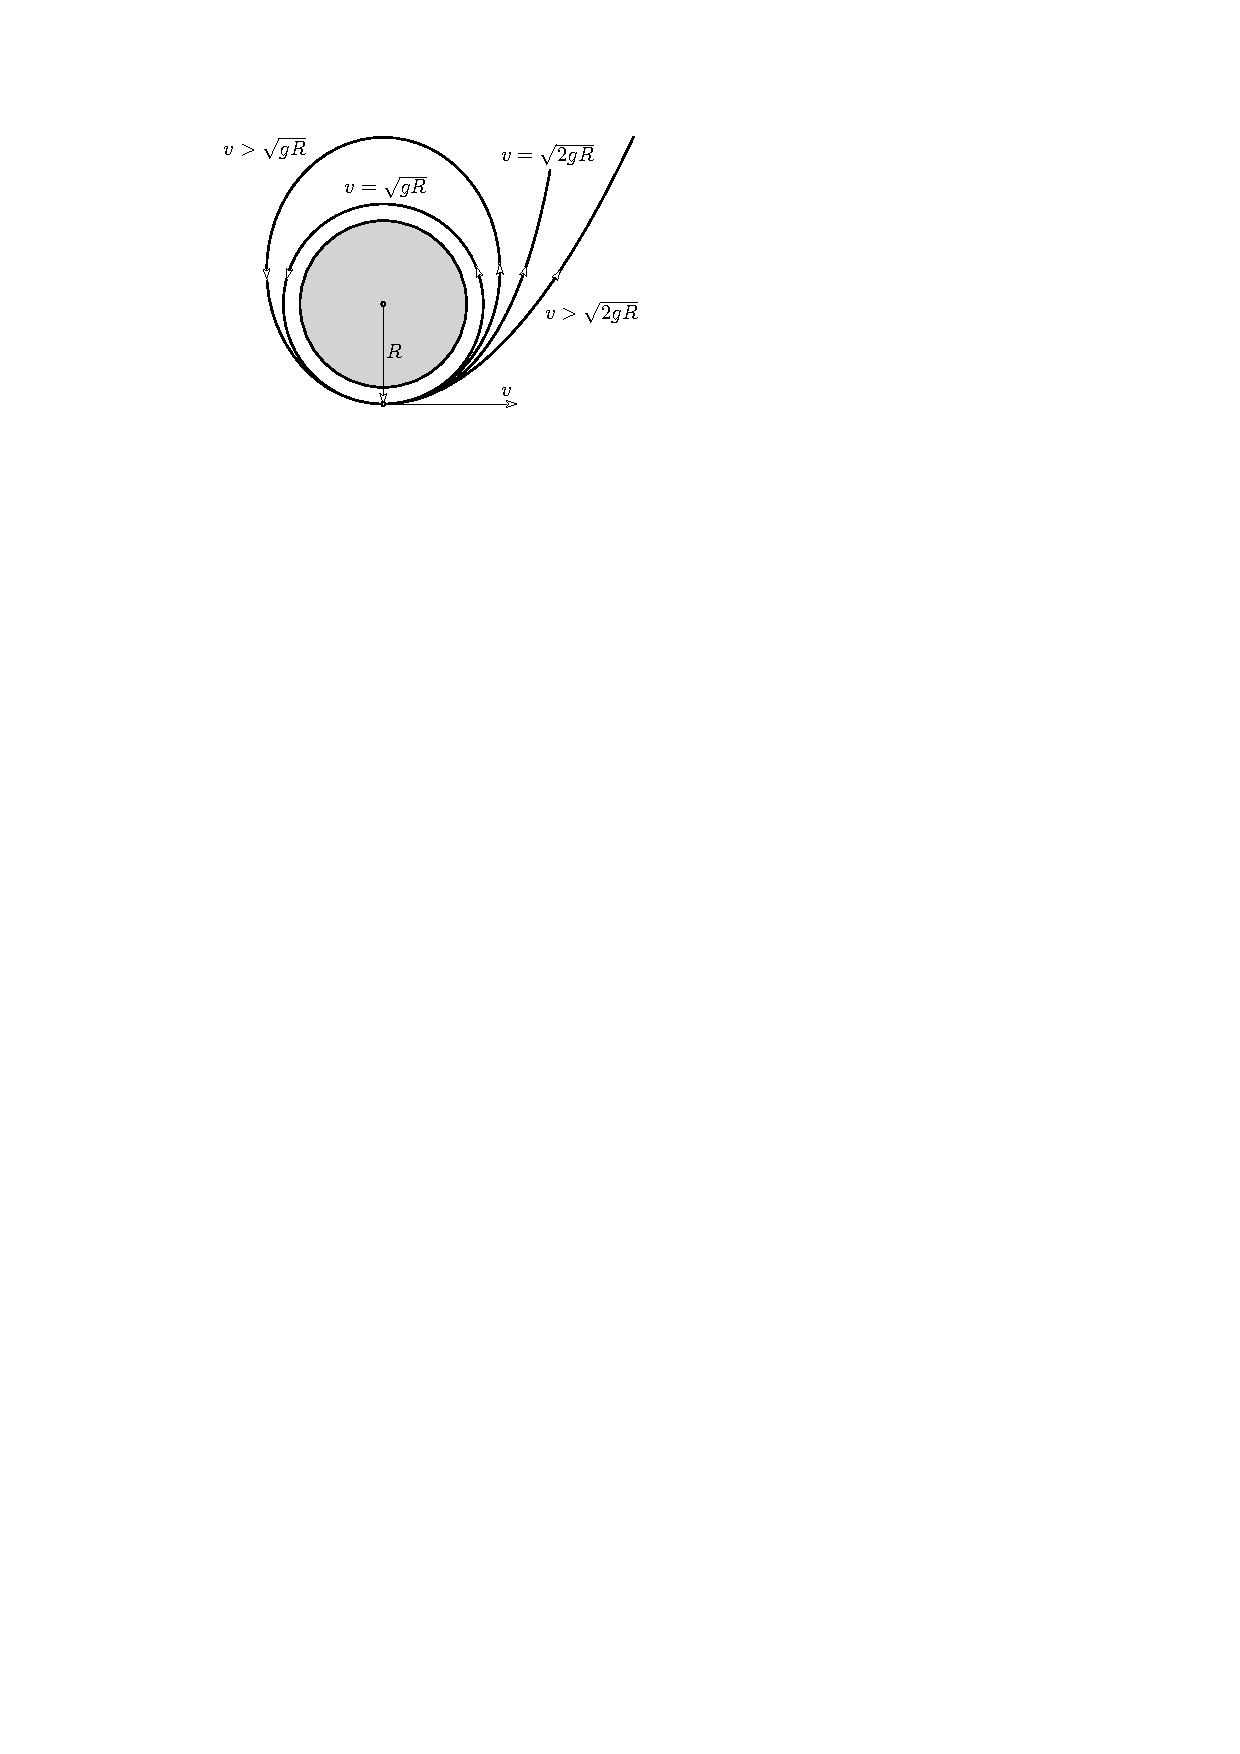
\includegraphics[width = 0.45\tw]{speeds}
	\caption{Возможные траектории тела \label{pic:orbits}}
\end{wrapfigure}
Если $E_0>0$, то траектория тела~--- \imp{гипербола},
ветви которой асимптотически приближаются к двум прямым. Стоит заметить,
что на бесконечно большом удалении малого \linebreak тела от массивного
его скорость остается положительной, так как суммарная энергия $E_0$
больше нуля.

Если $E_0=0$, то траектория тела~--- \imp{парабола}. При стремлении
расстояния $r$ между телами к бесконечности скорость тела с стремится к нулю.

Отсюда становится очевидно, что при параболической и гиперболической
траекториях движение тела не ограничено (инфинитно).

Если $E_0<0$, то траектория тела~--- \imp{эллипс}. При
эллиптической траектории движение ограничено (финитно), так как малое тело
не может бесконечно удаляться по причине того,
что суммарная энергия меньше нуля.

На Рис.\,\ref{pic:orbits} представлены примеры возможных траекторий малого тела
относительно центрального (точка C). При $v_0 > v_{2}$ тело движется
по гиперболе, при $v_0 = v_{2}$~--- по параболе,
а при $v_0 < v_{2}$~--- по эллипсу.

\term{Первая космическая скорость} --- минимальная скорость, необходимая для
того, чтобы маломассивное тело стало искусственным спутником центрального тела.
\begin{equation}v_1=\sqrt{\frac{GM}{R}},
\end{equation}
где $M$ --- масса центрального тела, а $R$~--- радиус орбиты. Отсюда несложно получить выражение для
скорости искусственного небесного тела на высоте~$h$ над~поверхностью тела радиуса $r_0$:
\begin{equation}
	v_h=\sqrt{\frac{GM}{r_0+h}}=\sqrt{\frac{g r_0^2}{r_0+h}}.
\end{equation}

\begin{wrapfigure}[10]{r}{.5\tw}
	\centering
	\vspace{-1pc}
%	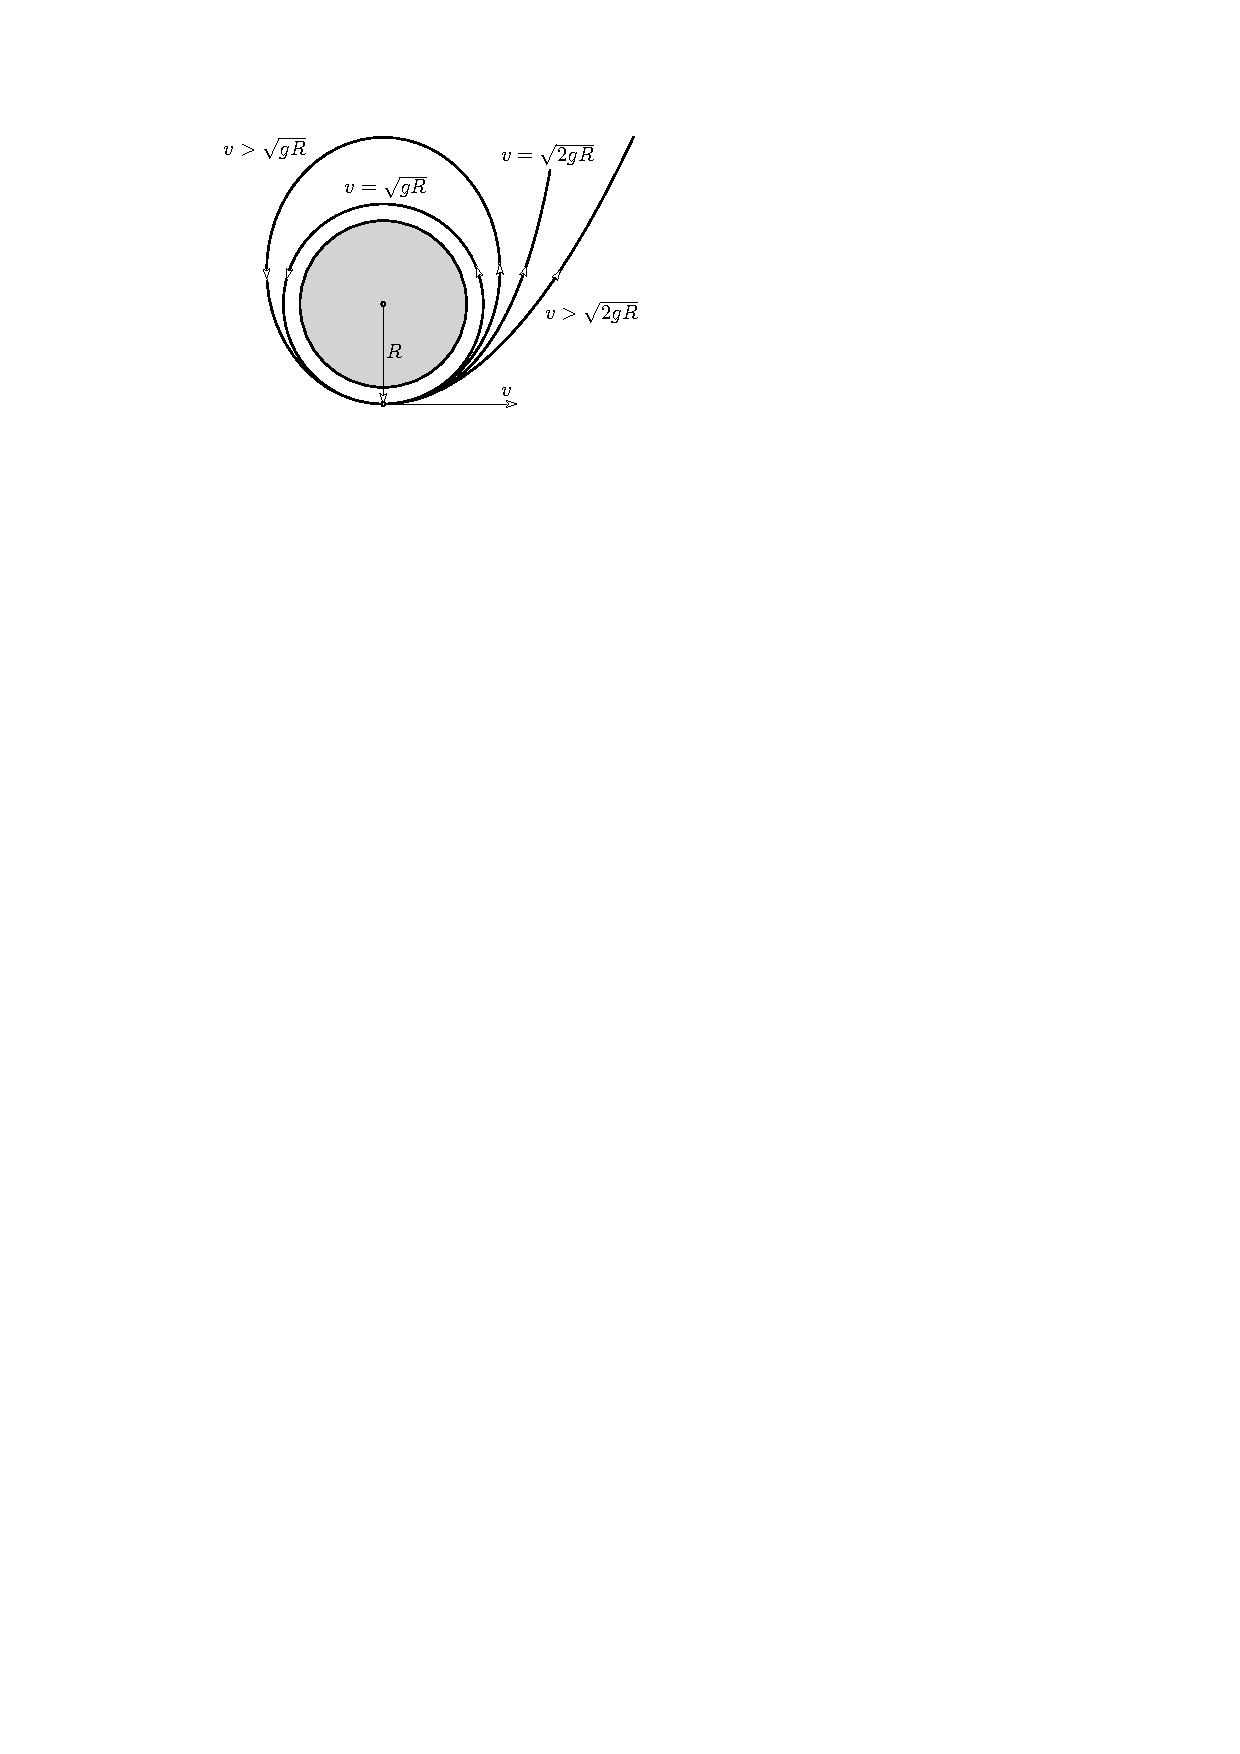
\includegraphics[width=.5\tw]{speeds}
	\caption{Движение по окружности \label{pic:orb-vel}}
\end{wrapfigure}
\change{Вывод:
\\
Рассмотрим 2 точки из траектории ($А$ и $В$) и скорости объекта в этих точках ($v_A$ и $v_B$) соответственно.
\begin{equation}
	\vec{\Delta v} = \vec{v_B} - \vec{v_A}
\end{equation}
При устремлении промежутка времени между пунктами к 0 можно считать, что длина пути становится равна длине хорды $AB$.
\begin{equation}
	\alpha = \frac{\Delta v}{v_A} = \frac{AB}{R}.
\end{equation}
Посчитаем модуль среднего ускорения:
\begin{equation}
	\langle a \rangle = \frac{\Delta v}{\Delta t} = \frac{v \Delta l}{R \Delta t}.
\end{equation}
Перейдя к пределу, получим мгновенное ускорение
\begin{equation}
	a = \lim_{\Delta t \rightarrow 0} \langle a \rangle = \lim_{\Delta t \rightarrow 0} \frac{v \Delta l}{R \Delta t} = \frac{v}{R} \lim_{\Delta t \rightarrow 0} \frac{\Delta l}{\Delta t} = \frac{v^2}{R}.
\end{equation}
Отсюда получаем значение для круговой скорости:
\begin{equation}
	v = \sqrt{a R} = \sqrt{\frac{G M}{R}}.
\end{equation}
}

\term{Параболическая} или \term{вторая космическая скорость} ---
минимальная скорость, необходимая для того, чтобы маломассивное тело преодолело гравитационное притяжение центрального тела, стартуя с расстояния $r$ от его центра масс, и покинуло замкнутую орбиту вокруг
последнего. Выражение для нее имеет следующий вид:
\begin{equation}
	v_{2}=\sqrt{\frac{2GM}{r}}.
\end{equation}